\documentclass[sigconf]{acmart}
% Cleaning
\pagestyle{fancy} % removes running headers
\settopmatter{printacmref=false} % Removes citation information below abstract
\renewcommand\footnotetextcopyrightpermission[1]{} % removes footnote with conference information in first column
\pagestyle{plain} % removes running headers
\fancyhead{}
\settopmatter{printacmref=false, printfolios=false}
% Copyright
\setcopyright{none}
\settopmatter{printacmref=false} % Removes citation information below abstract
\acmDOI{}

\usepackage{booktabs} % For formal tables
\usepackage{url}
\usepackage{algorithm}
\usepackage[noend]{algpseudocode}
\algtext*{EndWhile}% Remove "end while" text
\algtext*{EndIf}% Remove "end if" text
\algtext*{EndFor}% Remove "end for" text

\setlength{\parskip}{0pt}
\setlength{\parsep}{0pt}
\setlength{\headsep}{0pt}
\setlength{\topskip}{0pt}
\setlength{\topmargin}{0pt}
\setlength{\topsep}{0pt}
\setlength{\partopsep}{0pt}
\usepackage{mdwlist}
\usepackage{amsmath}
\usepackage{tikz}
\usetikzlibrary{positioning,arrows.meta}

\begin{document}
\title{Learning USV Drift from Telemetry: Linear, LSTM and Transformer Models}
\author{Jake Cushway}
\affiliation{
  \institution{University of Victoria}
  \city{Victoria}
  \country{Canada}
}
\email{jakecush1@uvic.ca}

\author{Rowan Hall}
\affiliation{
  \institution{University of Victoria}
  \city{Victoria}
  \country{Canada}
}
\email{rowanhall@uvic.ca}

\begin{abstract}
Between course corrections, the DataXplorer\texttrademark{} USV drifts with its motor off, and a pilot must step in before wind and current carry it out of its 10~nm station. We predict where the vessel will be one hour from now, using only its last hour of GPS track and wind. We define the task as regression and compare four models of increasing power (persistence, linear regression, LSTM, transformer), tested on a deployment they never saw. Code: \url{https://github.com/jakecush1/autonomous-pilot-ML} (\texttt{usv-intervention/v1\_ml/rowan}).\footnote{AI use (Guideline D): the code and a first draft of this paper were generated with Claude (Anthropic) and reviewed, run and edited by the authors.}
\end{abstract}

\keywords{Uncrewed surface vehicle, drift prediction, time series regression, LSTM, transformer}
\maketitle
\pagestyle{empty}

\section{Introduction}\label{sec:intro}
The Open Ocean Robotics DataXplorer replaces a retired NOAA weather buoy and must stay within 10~nm of the buoy's old position. It mostly drifts with the motor off, and a shore pilot watches it around the clock although a correction is needed only every few hours. In Milestone~2 we proposed predicting \emph{when} the pilot must act. The first building block is predicting \emph{where} the drifting vessel is going: a predicted position an hour ahead can be checked against the boundary to warn the pilot early. Unlike drift models built on physics and weather forecasts~\cite{dugan2024drifting,song2024drift}, we learn drift directly from the vessel's own logged telemetry. We contribute a formal task definition, a leak-free data pipeline, and a comparison of four models.

\section{Problem Definition}\label{sec:problem}
\emph{In words: given the last hour of a drifting vessel's track and wind, predict how far it will move east and north in the next hour.}

A deployment is a sequence of 1-minute telemetry records $\mathcal{S}=\{s_\tau\}_{\tau=1}^{T}$, where $s_\tau=(\phi_\tau,\lambda_\tau,v_\tau,\theta_\tau,m_\tau)$ holds latitude, longitude, wind speed (kn), the compass direction the wind comes \emph{from}, and motor power (W). The vessel is \emph{drifting} at minute $\tau$ if $m_\tau=0$. Let $\mathbf{p}_\tau\in\mathbb{R}^2$ be its position in metres east and north of the station (\S\ref{sec:repr}). For a time $t$ at which the vessel has drifted for the past $H$ minutes, our solution is a function
\begin{equation}\label{eq:f}
f:\mathbb{R}^{H\times 4}\rightarrow\mathbb{R}^{2},\qquad \hat{\mathbf{y}}_t=f(\mathbf{X}_t)\approx\mathbf{y}_t=\mathbf{p}_{t+H}-\mathbf{p}_t,
\end{equation}
where $\mathbf{X}_t$ describes the past $H$ minutes (4 numbers per minute) and $\mathbf{y}_t$ is the movement over the next $H$ minutes, assuming the motor stays off. The predicted position is $\hat{\mathbf{p}}_{t+H}=\mathbf{p}_t+\hat{\mathbf{y}}_t$. The output is a distance, not a category, so this is regression rather than classification. We use $H=60$.

\section{Proposed Approach}\label{sec:approach}
Figure~\ref{fig:pipeline} shows the pipeline and Algorithm~\ref{alg:drift} gives the pseudo-code.

\subsection{Representation}\label{sec:repr}
\textbf{Position.} GPS degrees are converted to metres from the station centre $(\phi_0,\lambda_0)$, so that distances and movements are meaningful: $\mathbf{p}_\tau=R\,\big((\lambda_\tau-\lambda_0)\cos\phi_0,\;\phi_\tau-\phi_0\big)$, with $R=6371$\,km and angles in radians. This flat-earth approximation is off by less than 0.3\% within 10~nm.
\textbf{Wind.} The wind blowing \emph{from} direction $\theta$ pushes the vessel the opposite way, so we use the push vector $\mathbf{w}_\tau=-v_\tau(\sin\theta_\tau,\cos\theta_\tau)$ (east, north). Using sine and cosine also avoids the jump from 359° to 0°.
\textbf{Input window.} For each minute we keep its movement $\Delta\mathbf{p}_\tau=\mathbf{p}_\tau-\mathbf{p}_{\tau-1}$ and the wind push, giving
$\mathbf{X}_t=[\,(\Delta\mathbf{p}_\tau,\mathbf{w}_\tau)\,]_{\tau=t-H+1}^{t}$, a table of 60 rows by 4 columns.

\subsection{Cleaning and Splitting the Data}
Gaps of up to 5 missing minutes are filled by linear interpolation. A minute is \emph{valid} if the motor is off, no value is missing, and the vessel moved less than 93\,m (about 3\,kn; faster means it was being towed, not drifting). A time $t$ becomes a training sample $(\mathbf{X}_t,\mathbf{y}_t)$ only if all 120 minutes from $t-59$ to $t+60$ are valid, so neither the input nor the answer includes motor use. Five deployments (Apr--Oct 2026, 85{,}910 minutes) give 23{,}319 samples.

Samples one minute apart share 59 of their 60 input minutes, so a random train/test split would put near-copies of test samples in training. We therefore split by whole deployment: \textbf{train} (Apr, May--Jun, Aug; 16{,}471 samples), \textbf{validation} (Oct 3--13; 2{,}289), used only to decide when to stop training, and \textbf{test} (Oct 16--23; 4{,}559), never used for any choice. Inputs and targets are rescaled to mean 0 and standard deviation 1 using training data only.

\subsection{Models}
Each model is a different way to compute $f$ in Eq.~\ref{eq:f}.
\textbf{(1) Persistence} (baseline, no training): the next hour repeats the last, $\hat{\mathbf{y}}_t=\sum_{\tau}\Delta\mathbf{p}_\tau$. Drift is driven mostly by current and tide, which change slowly, so this is a strong bar to beat.
\textbf{(2) Linear regression}: $\hat{\mathbf{y}}_t=\mathbf{A}\,\mathbf{z}_t+\mathbf{c}$, where $\mathbf{z}_t$ summarises the window in 6 numbers (past-hour movement, current wind push, mean wind push over the hour) and $\mathbf{A}\in\mathbb{R}^{2\times6}$, $\mathbf{c}$ are fitted by least squares. It tests whether a fixed weighting of drift and wind helps, and its weights can be read directly.
\textbf{(3) LSTM}~\cite{hochreiter1997lstm}: reads the 60 rows of $\mathbf{X}_t$ one minute at a time, updating a memory vector $\mathbf{h}$; the final $\mathbf{h}_t$ is mapped to $\hat{\mathbf{y}}_t=\mathbf{W}\mathbf{h}_t+\mathbf{b}$. Unlike the 6-number summary, it can see whether the drift is turning or slowing down.
\textbf{(4) Transformer}~\cite{vaswani2017attention}: each minute becomes a 64-number vector plus a code for its position in time, $\mathbf{e}_\tau=\mathbf{W}_e\mathbf{x}_\tau+\mathrm{PE}(\tau)$. Self-attention layers let every minute compare itself with every other; the outputs are averaged over the hour and mapped to $\hat{\mathbf{y}}_t$.

The models go from simplest to most flexible; a more complex one is only worth using if it beats the simpler one on unseen data. Sizes are in Table~\ref{tab:hparams}.

\subsection{Training, Inference and Scoring}
The LSTM and transformer minimise mean squared error with Adam~\cite{kingma2015adam}. After each pass over the training data (epoch) we keep the weights with the lowest validation loss and stop after 10 epochs without improvement. This matters because the 23k overlapping windows hold only about 400 independent hours of drift, and both networks start memorising within a few epochs. Settings are common defaults, not tuned; tuning is part of Milestone~4. At inference the output is scaled back to metres and added to $\mathbf{p}_t$.

We score each prediction by its \textbf{endpoint error} $e_t=\|\hat{\mathbf{p}}_{t+H}-\mathbf{p}_{t+H}\|_2$, the distance in metres between predicted and true position, since distance is what matters to the pilot. We report the median (a typical miss, robust to GPS glitches) and the 90th percentile (a bad-case miss, usable as a safety radius).

\textbf{Worked example.} On Oct 19 at 21:15 (test deployment) the vessel had moved $(774, 555)$\,m east/north in the past hour, slowing down, with a light 4\,kn wind. Persistence predicts the same $(774, 555)$\,m again; the trained LSTM predicts $(460, 353)$\,m; the vessel actually moved $(283, 194)$\,m. The endpoint errors are 609\,m for persistence and 238\,m for the LSTM, which noticed the slowdown.

\begin{table}[t]
\caption{Hyperparameters (top-level constants in the code).}
\label{tab:hparams}
\footnotesize
\begin{tabular}{@{}ll@{}}
\toprule
LSTM & 2 layers, 64 hidden units, dropout 0.2 \\
Transformer & width 64, 4 heads, 2 layers, feed-forward 256, dropout 0.1 \\
Training & Adam, learning rate $10^{-3}$, batch 256, gradient clip 1.0 \\
Stopping & $\leq$80 epochs, patience 10 on validation loss; seed 0 \\
\bottomrule
\end{tabular}
\end{table}

\begin{algorithm}[t]
\caption{Drift prediction: build data, train, predict}
\label{alg:drift}
\begin{algorithmic}[1]
\Statex\textbf{Input:} deployments $\{\mathcal{S}_k\}$, horizon $H$, model $f_\Theta$
\Statex\textbf{Output:} trained $f_{\Theta^*}$; predicted position $\hat{\mathbf{p}}_{t+H}$
\ForAll{deployments $\mathcal{S}_k$} \Comment{build samples}
\State fill gaps $\leq5$ min; $\mathbf{p}_\tau\gets$ metres from centre
\State $\mathbf{w}_\tau\gets-v_\tau(\sin\theta_\tau,\cos\theta_\tau)$ \Comment{wind push}
\State valid$_\tau\gets$ motor off $\land$ no missing $\land\ \|\Delta\mathbf{p}_\tau\|<93$
\ForAll{$t$ where minutes $t{-}H{+}1..t{+}H$ are all valid}
\State add $(\mathbf{X}_t,\ \mathbf{y}_t=\mathbf{p}_{t+H}-\mathbf{p}_t)$ to the split of $\mathcal{S}_k$
\EndFor
\EndFor
\State rescale with train statistics; seed $\gets0$; best $\gets\infty$
\For{epoch $=1..80$} \Comment{train}
\ForAll{mini-batches $B$ of train}
\State $\Theta\gets\mathrm{Adam}\big(\Theta,\nabla_\Theta\tfrac{1}{|B|}\sum_{B}\|f_\Theta(\mathbf{X})-\mathbf{y}\|^2\big)$
\EndFor
\If{val loss $<$ best} best $\gets$ val loss; $\Theta^*\gets\Theta$
\ElsIf{no improvement for 10 epochs} \textbf{break}
\EndIf
\EndFor
\State \Return $\hat{\mathbf{p}}_{t+H}=\mathbf{p}_t+f_{\Theta^*}(\mathbf{X}_t)$ \Comment{predict}
\end{algorithmic}
\end{algorithm}

\begin{figure}[t]
\centering
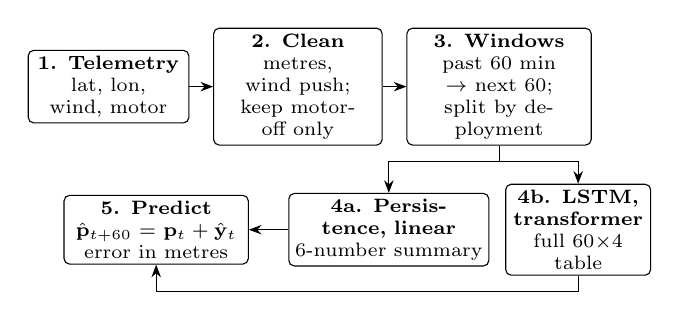
\begin{tikzpicture}[font=\scriptsize, node distance=4mm and 3mm,
  box/.style={draw, rounded corners=2pt, align=center, minimum height=7mm, inner sep=2pt, text width=#1},
  box/.default=20mm,
  arr/.style={-{Stealth[length=1.6mm]}}]
\node[box=19mm] (raw) {\textbf{1. Telemetry}\\lat, lon, wind, motor};
\node[box=20mm, right=of raw] (pre) {\textbf{2. Clean}\\metres, wind push;\\keep motor-off only};
\node[box=22mm, right=of pre] (win) {\textbf{3. Windows}\\past 60 min $\rightarrow$ next 60;\\split by deployment};
\node[box=24mm, below=6mm of win, xshift=-14mm] (lin) {\textbf{4a. Persistence, linear}\\6-number summary};
\node[box=17mm, right=2mm of lin] (seq) {\textbf{4b. LSTM,}\\\textbf{transformer}\\full 60$\times$4 table};
\node[box=22mm, left=5mm of lin] (out) {\textbf{5. Predict}\\$\hat{\mathbf{p}}_{t+60}=\mathbf{p}_t+\hat{\mathbf{y}}_t$\\error in metres};
\draw[arr] (raw) -- (pre);
\draw[arr] (pre) -- (win);
\draw[arr] (win.south) -- ++(0,-2mm) -| (lin.north);
\draw[arr] (win.south) -- ++(0,-2mm) -| (seq.north);
\draw[arr] (lin) -- (out);
\draw[arr] (seq.south) -- ++(0,-2mm) -| (out.south);
\end{tikzpicture}
\caption{Pipeline: telemetry is cleaned and cut into 60-minute motor-off windows; each model maps a window to the next 60 minutes' movement.}
\label{fig:pipeline}
\end{figure}

\section{Implementation}\label{sec:impl}
The code is in Python (scikit-learn, PyTorch), one file per pipeline stage, matching Algorithm~\ref{alg:drift}: \texttt{data\_prep.py} (representation, cleaning, split, endpoint error; lines 1--6), \texttt{linear\_reg.py} (persistence, linear regression), \texttt{nn\_models.py} (LSTM, transformer, training loop; lines 7--13) and \texttt{compare.py} (results table, chart). Outputs go to \texttt{outputs/}. The README covers the project, installation, quick start and results; dependencies are pinned in \texttt{requirements.txt} and the data are in the repository. The quick-start script \texttt{quickstart.sh} creates the environment on first use and runs all five steps in order (about 5 minutes on a laptop CPU):
{\footnotesize
\begin{verbatim}
git clone https://github.com/jakecush1/autonomous-pilot-ML
cd autonomous-pilot-ML/usv-intervention/v1_ml/rowan
bash quickstart.sh
\end{verbatim}}
\textbf{Reproducibility.} Seeds are fixed to 0 and the split is fixed by deployment, so the quick start on CPU reproduces Table~\ref{tab:results} exactly (confirmed on three runs).

\begin{table}[t]
\caption{First run: endpoint error after 60 min, unseen test deployment.}
\label{tab:results}
\footnotesize
\begin{tabular}{@{}lccc@{}}
\toprule
Model & Median (m) & 90th pct. (m) & $R^2$ \\
\midrule
No drift ($\hat{\mathbf{y}}=0$) & 586 & 1515 & 0.00 \\
(1) Persistence & 294 & 570 & 0.80 \\
(2) Linear regression & 318 & 631 & 0.77 \\
(3) LSTM & 247 & 497 & 0.85 \\
(4) Transformer & \textbf{246} & \textbf{477} & \textbf{0.86} \\
\bottomrule
\end{tabular}
\end{table}

\textbf{First results.} Table~\ref{tab:results} shows the pipeline runs end to end. Persistence already halves the error of assuming no drift. Linear regression does \emph{not} beat persistence on the unseen deployment, while the LSTM and transformer both do, by about 16\%, and are tied with each other. Milestone~4 will test more seeds and horizons and turn the prediction into a time until the vessel reaches the boundary~\cite{dugan2024drifting}, toward an intervention probability~\cite{kristensen2022dynamic}.

\bibliographystyle{ACM-Reference-Format}
\bibliography{bibliography.bib}

\end{document}
